%-------------------------------------------------------------------------------------------------------------------
% THE PROBLEM OF IMBALANCED DATASETS
%-------------------------------------------------------------------------------------------------------------------
\chapter{Classification in Imbalanced Datasets}\label{imbalanced}
Previous chapter discussed how the classification task can be solved in machine learning. However, a successful solution to this task can be seriously hindered. For example, complications can arise when when we have class imbalanced data: a class of interest is heavily under-represented in comparison to other classes. This problem and its implications are described in section~\ref{imbalanced-theproblem} and~\ref{causestheproblem}. Although no global solution has yet been found, many approaches have been introduced during the past decade. We discuss some of these approaches in section~\ref{approaches}. Finally, we finish in section~\ref{imb-summary} with a conclusion.


\section{Problem Description}\label{imbalanced-theproblem}
An imbalanced (or skewed) dataset occurs when a class of interest is heavily under-represented in comparison to the other classes.  These kind of datasets occur in many applications, such as medical diagnosis/monitoring, fraud/intrusion detection, text categorization, risk management, information retrieval and filtering tasks.  Moreover, when the data collection process is limited or very time consuming, it might happen that class imbalances occur in domains that do not have an intrinsic imbalance.  Typical, the ratio of the small to the large class takes proportions such as 1 to 100, 1 to 1\,000, 1 to 10\,000 or even more. Since many standard classifiers try to maximize accuracy and do not alter the distribution from the training data, they tend to be overwhelmed by the large classes and ignore the small ones~\cite{ProvostMLID}. The reason why should be clear: predicting the majority class in imbalanced datasets will easily yield accuracies of more than 99\%. 

%-------------------------------------------------------------------------------------------------------------------
% Implications of Class Imbalance
%-------------------------------------------------------------------------------------------------------------------
\section{Class Imbalance, Noise, and Outliers}\label{causestheproblem}
Class imbalance is mainly related to rarity, of which two different situations can occur. The first type of rarity is called \textit{rare classes}, and concerns the poor presence of instances of a specific class. The second type of rarity concerns \textit{rare cases}, which correspond to a meaningful but relatively distant cases of the classes. For simplicity, we call this rare cases \textit{outliers}. Although rare classes and outliers are not directly related, empirical studies show that the minority class contains a greater proportion of outliers than the majority class~\cite{Weiss03learningwhen}. Since in many situations outliers cannot be distinguished from class noise, recognizing more (less) outliers more likely results into overfitting (underfitting) the minority class. Besides class noise, the existence of feature noise can significantly influence the distribution of the minority data. When feature noise occurs in minority class clusters, affected instances can become outliers. On the other hand, when feature noise occurs in outliers, affected instances can disappear within the minority class clusters. Hence, recognizing more (less) outliers may again result into overfitting (underfitting). When the minority data is scattered, feature noise does not have this effect.~\cite{Japkowicz02classimbalance}~\cite{Prati04classimbalances}~\cite{miningwith04}


%-------------------------------------------------------------------------------------------------------------------
% CURRENT SOLUTIONS
%-------------------------------------------------------------------------------------------------------------------
\section{Approaches}\label{approaches}
In order to overcome the class imbalance problem, many approaches have been introduced. The most famous approaches try to tackle the lack of the minority data by increasing their number through sampling (section~\ref{sampling-techniques}) or cost-sensitivity (section~\ref{cost-sensitivity}). Other approaches try to identify the minority objects, rather than the separation between the minority and the majority data (section~\ref{one-class}). Classifier improvements can also be obtained by altering the feature selection process in learning algorithms such as CART or C4.5. Often, measures used in this process are based on unreliable estimates or favor the recognition of the majority class. We discuss some improvements for these measures and estimates in section~\ref{feat-select}. More improvements can be obtained by using different evaluation metrics, as many of them do not value rarity well. However more appropriate metrics have already been discussed, we give a short summary in section~\ref{app-eval-metric}. A last approach considers combining a set of classifiers (also called a classifier ensemble), with the goal to obtain more reliable predictions than a single classifier (section~\ref{classif-ensembles}). 



\subsection{Sampling techniques}\label{sampling-techniques} 
Sampling is probably the most-direct approach to handle class imbalances. It changes the priors in the training set by either increasing instances from the minority class (\textit{over-sampling}), decreasing instances from the majority class (\textit{under-sampling}), or a combination of both. As a result, the class distribution of the training data is changed such that the resulting data is more balanced. Although general implementation is fairly simple, some disadvantages threaten its use.  First of all, under-sampling might discard useful data, what would lead to under-fitting the (majority class) data. On the other hand, over-sampling might result into overfitting the (minority class) data, since most over-sampling methods generate exact copies of existing instances. Moreover, over-sampling increases the size of the training set, which will increase the time necessary to learn the classifier~\cite{mccarthy}.

Sampling techniques are a direct approach to tackle with class imbalances, and can be used in combination with any classifier. Moreover, under-sampling allows a solution to the enormous data sets which size needs to be reduced.  Finally, the use of sampling rates allows the fine-tuning of class imbalances, and therefore their resulting classification models and performance.  

\subsubsection{Monte Carlo Sampling}
Monte Carlo methods were introduced in 1949 by Metropolis and Ulam~\cite{Metropolis49MonteCarlo}, and are a class of computational algorithms that rely on repeated random sampling in order to perform a specific task. In the context of over-sampling, the goal is to generate samples from the minority distribution. This can for example be achieved by sampling with replacement from the minority distribution, a technique known as bootstrapping. In the same way, bootstrapping can be used to under-sample the majority distribution.

An important example of Monte Carlo sampling is the Gibbs sampling algorithm. Gibbs sampling generates a sequence of samples from the joint probability distribution of two or more random variables. The purpose is to approximate the joint distribution, or to compute an integral (such as expected value).  Gibbs sampling was introduced by Stuart German \& Donald German~\cite{Stochastic84} in the context of image processing and then discussed in the context of missing data problems by Tanner \& Wong~\cite{calcpost87}. Gibbs sampling is applicable when the joint distribution is not known explicitly, but the conditional distribution of each variable is known.  The Gibbs sampling algorithm generates an instance from the distribution of each variable in turn, conditional on the current values of the other variables.  It can be shown that the sequence of samples constitutes a Markov chain, and the stationary distribution of that Markov chain is just the sought-after joint distribution. 

Other extensions which are related to Monte Carlo methods are Rejection sampling, Importance sampling, Gibbs sampling and Slice sampling~\cite{bishop}~\cite{Neal03slicesampling}.

\subsubsection{SMOTE}\label{smote}
\index{sampling techniques!SMOTE}
Synthetic minority over-sampling technique (SMOTE) was introduced by Cieslak \& Chawla, who suggest a local implementation of sampling based on the belief of multi-modality of many datasets~\cite{StartGlobally08}~\cite{smote}.  Instead of over-sampling with replacement, SMOTE creates "synthetic" instances along the line segments joining any/all of the \textit{k} minority class nearest neighbors. Hence, SMOTE is a generative sampling model. Since generated instances are strongly related to existing instances, this approach forces the decision region of the minority class to become more general (avoid overfitting).  When combined with under-sampling, SMOTE tends to improve overall performance compared to over-sampling with replacement.  Although implementation increases computational cost of the learning algorithm, experiments have shown the convenience of applying SMOTE when the data set has very few positive (minority) instances~\cite{batista}.



\subsection{Cost-sensitive Learning}\label{cost-sensitivity}
\index{costsensitive learning}
Another approach to deal with imbalanced datasets, is to introduce cost-sensitivity during the training or evaluation of a classifier. This allows the classifiers to focus more on predicting specific classes, and can be achieved by assigning costs to each type of (mis)classification. Usually, these costs are accepted as user input and learned by comparing various cost settings. The set of assigned costs for a classifier is often given by a \textit{cost matrix}, and looks as follows:

\begin{table}[h]
\centering                            % centering table
\begin{tabular}{|l| c| c c c c|}              % creating 10 columns
\hline                                % inserting double-line
& & \multicolumn{4}{|c|}{Actual} \\
\hline 
& & Class 1 & Class 2 & & Class $\mathbf{Y}$\\ [0.5ex]
\hline                                      % inserts single-line
& Class 1 & $CM_{11}$ & $CM_{12}$ & \ldots & $CM_{1|\mathbf{Y}|}$ \\
& Class 2  & $CM_{21}$  &  $CM_{22}$  & \ldots & $CM_{2|\mathbf{Y}|}$ \\
\raisebox{1.5ex}{Predicted}  & & \raisebox{1.5ex}{\ldots} & \raisebox{1.5ex}{\ldots}  & & \raisebox{1.5ex}{\ldots} \\
& Class $\mathbf{Y}$ &  $CM_{|\mathbf{Y}|1}$ & $CM_{|\mathbf{Y}|2}$ & \ldots & $CM_{|\mathbf{Y}||\mathbf{Y}|}$ \\
\hline                          % inserts single-line
\end{tabular}
\label{tab:PPer}
\end{table}

Summarized, a cost matrix describes the cost of classifying an object of class $i$ (actual class) as class $j$ (predicted class) in entry $CM_{ij}$. Since misclassifying is costly, usually $CM_{ij} \geq 0$ if $i \neq j$, and, since correct classification does not cost anything, $CM_{ij}  = 0$ if \(i = j\). However, some classifiers induce a gain (negative cost) $CM_{ij} \leq 0$ for correctly classifying instances in order to quantify the consequences of a good classification.

In a 2-class classification problem (where the second class describes the minority data), the cost assignments are usually the following:
\begin{itemize}
\item $CM_{11} = CM_{22} = 0$
\item $CM_{21} = 1$
\item $CM_{12} > 1$
\end{itemize}

Cost-sensitive learning employs the cost-sensitive matrix. There are different scenarios given below:

\begin{itemize}
\item \textbf{Clasifier evaluation}: an easy solution to implement costs is to apply them in the classifier evaluation. An \textit{expected misclassification cost} can be calculated by making a cross-product between the misclassification cost matrix and the confusion matrix, which allows comparison of models.
\item \textbf{Minimizing expected cost}: in this approach, the costs are handled during the learning process. The classifier is trained without considering the costs, but uses a classification rule that minimizes the expected loss. Conditional probabilities provided by the model are used to calculate the loss associated with each decision, and the decision which minimizes the expected loss is then chosen. The main advantage of this approach is that it allows to use, without specific modifications, the results provided by the classifier output.
\item \textbf{Instance reweighting}: this approach will assign a weight to each training instance according to its misclassification cost, and can therefore be compared to sampling techniques, with the difference that the number of instances does not change.
\item \textbf{Class probability thresholds}: some classifiers, such as the Naive Bayes classifier or some Neural Networks, yield a score that represents the degree to which an instance is a member of a class.  In such cases, altering the threshold which decides whether the instance is labeled as positive or negative, can produce several classifiers. For example, classifiers generally use 0.50 as threshold value, meaning that if the classifier output for a specific instance is above 50\%, the classifier produces a \textbf{Y}, else a \textbf{N}.  If this threshold value is now altered to 0.60, a different classifier will be obtained.  This technique is used in the construction of ROC graphs~\cite{roc}.
\end{itemize}
Results of a comparative study~\cite{mccarthy} show that cost-sensitive learning and over-sampling perform similarly whereas under-sampling performs much worse.  When datasets are very large, cost-sensitive learning seems to outperform other techniques, perhaps because the larger amount of training data makes it easier to estimate more accurately the class-membership probabilities.  However, although cost-sensitivity allows a flexible solution to class imbalances, recent studies have shown that clever re-sampling and combination methods can do more than cost-sensitive learning as they provide new information or eliminate redundant information for the learning algorithm.~\cite{Chawla04editorial:special}


\subsection{One-Class Learning}\label{one-class}
One-class learning is a different approach which proves particularly useful on extremely imbalanced data sets with a high-dimensional noisy feature space~\cite{raskutti}. As recognition-based approach, it learns a classifier which can predict samples of one (usually the minority) class.  Therefore, this approach differs from sampling and cost-sensitivity since it does not consider the class imbalance as a problem. It focuses on the separation between the minority and the majority classes.

There are two main strategies for one-class learning. The first one tries to recognize instances of the (usually) minority class rather than discriminate between instances of all classes. As a result, the goal of this strategy is to define a boundary around the target class such that as many objects as possible of the target classes are recognized, while a minimal amount of outliers are accepted. 
The second approach to one-class learning uses instances of both classes to make predictions about the target class, and uses internal bias strategies during the learning process to achieve this goal~\cite{one-class-classification}~\cite{REMED}.

An example of the first approach to one-class learning is Rule Extraction for MEdical Diagnosis (REMED)~\cite{REMED}. This approach is designed to deal with the imbalanced class problem, and to provide predictions with a reliability measure. REMED is a symbolic one-class approach to solve binary classification tasks. It is trained with instances of both classes and implements internal strategies during the learning process to maximize the correct prediction of the minority class instances. In general, REMED generates rule systems which are supported by attribute selection based on simple logistic regression to test the association and its confidence (99\% or 99.99\%) with the studied disease.

An example of the second approach to one-class learning can be found in so-called \textit{separate-and-conquer rule learning} or \textit{covering algorithms}~\ref{sepandconq}. These algorithms basically search for a rule that explains a part of the training instances, separate them and recursively conquer the remaining instances by learning more rules until no instances remain. As a result, they do not necessarily focus on one class. Since this technique can easily lead into overfitting, constraints are often relaxed by the use of stopping criteria and/or post-processing methods~\cite{sepandconq}. A typical covering algorithm is RIPPER, which generates rules for each class from the minority class to the majority class~\cite{jrip}~\cite{Kotsiantis06}.


\subsection{Feature Selection}\label{feat-select}
Many learning algorithms such as decision tree learning employ feature selection in order to build a classifier (see section~\ref{classifier-example}). The main idea of feature selection is to choose a subset of input features by eliminating features with little or no predictive information according to some measure. As a result, feature selection has a significant influence on the inductive bias of the classifiers. To adopt feature selection within the imbalanced problem, there exist two approaches. The first one is based on adapting class-probability estimates. The second approach is based on the introduction of new feature selection measures. 

To adapt feature selection measures (such as Information Gain), we can modify the way we estimate the class-probabilities. For example, if there are \(N_i\) instances of a class \(i\) at a leaf and \(|\mathbf{Y}|\) classes, then the probability that an instance at the leaf is a member of class \(i\) is given by:

\begin{eqnarray}
&&\hat{P}(y_i|x) = \frac{N_i}{\sum_{j=1}^{|\mathbf{Y}|}{N_j}}
\end{eqnarray}

When data is sparse, this estimate can be very unreliable. For this reason, several smoothing techniques have been introduced to improve the quality of the estimates. 

The Laplace estimate smooths the probability estimates by introducing a prior probability \(1/|\mathbf{Y}|\)~\cite{probest06}:

\begin{eqnarray}
&&\hat{P}(y_i|x) = \frac{N_{i}+1}{|\mathbf{Y}| + \sum_{j=1}^{|\mathbf{Y}|}{N_j}}
\end{eqnarray}

However, Laplace estimates might not be very appropriate for highly imbalanced datasets (Zadrozny \& Elkan 2001).  In those cases, it could be useful to incorporate the prior of positive class to smooth the probabilities so that the estimates are shifted towards the minority class base rate.  

A more general estimate than the Laplace estimate, is the so-called m-estimate. This estimate uses a parameter \(m\) which controls the role of the prior probabilities \(b_i\) of the considered class \(i\) and the evidence provided by the instances.

\begin{eqnarray}
&&\widehat{P}(y_i|x) = \frac{N_{i}+mb_i}{m + \sum_{j=1}^{|\mathbf{Y}|}{N_j}}
\end{eqnarray}

Higher values for \(m\) give more weight to the prior probabilities and less to the instances, therefore appropriate for datasets that contain more noise. The prior \(b_i\) can be estimated from the training set using relative frequency. We note that the Laplace estimate is a special case obtained by setting \(m\) to \(|\mathbf{Y}|\), and \(b\) to \(1/|\mathbf{Y}|\) for all classes (uniform distribution).

Another approach to improve the quality of the estimates was introduced by Nitesh \& Chawla~\cite{probest06}. They propose an ensemble method to smooth out the probability estimates at the leaves by bagging decision trees. The different estimates for $\hat{P}(y_i|x)$ are averaged, therefore improving the quality of the estimates and reducing the variance.\\

In stead of improving the probability estimates, one can also try to improve the actual measure used for feature selection. A typical measure used in decision tree learning is Information Gain, which uses entropy to characterize the impurity of an arbitrary set of instances. The problem with this (and many other) measure is that it associates most of the features in imbalanced datasets with the majority class~\cite{Zheng04featureselection}.

In order to overcome this problem, Cieslak \& Chawla proposed a variant of Hellinger distance (which is a measure of distributional divergence) as a new measure for feature selection. This measure mainly captures the divergence between feature values given two or more different classes. Since the prior does not influence the distance calculation, Hellinger distance is a skew insensitive measure.~\cite{hellinger}. 

Assuming a two-class problem, its calculation is based on the class-within presence of positive and negative instances compared to their overall presence.  Since Hellinger distance does not take the distribution over the classes into consideration, it favours the recognition of minority classes.

\begin{figure}[h]
\centering
\subfloat[10000:10000]{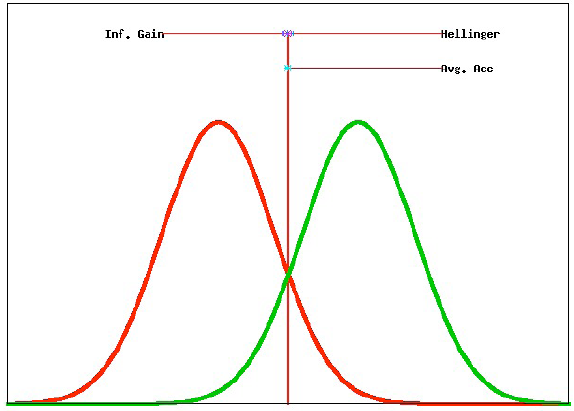
\includegraphics[scale=0.35]{img/Hellinger_01.png}}                
\subfloat[1000:10000]{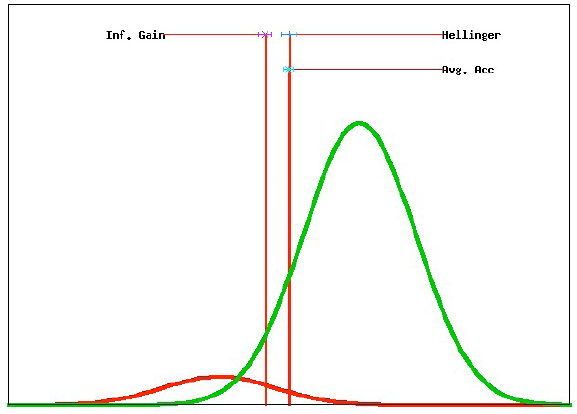
\includegraphics[scale=0.35]{img/Hellinger_02.png}}  
\caption{The effect of class imbalance (figure b) on the measures Information Gain and Hellinger distance.}
\end{figure}

In a two-class problem, let \(S_1\) be a sample of class 1 and \(S_2\) be a sample of class 2. Assuming the sample \(S\) is distributed over \textit{p} partitions in a certain feature, the Hellinger distance between \(S_1\) and \(S_2\) within that feature is defined as follows:

\begin{eqnarray}
&&Hellinger \left (S,S_1,S_2 \right)=\sqrt{\sum_{j=1}^p {\left(\sqrt{\frac{|\mathbf{S}_{1j}|}{|\mathbf{S}_1|}} - \sqrt{\frac{|\mathbf{S}_{2j}|}{|\mathbf{S}_2|}} \right )^2}}
\end{eqnarray}

where \(S_k\) stands for the number of instances of class \(k\) and \(S_{kj}\) for the number of instances of class \(k\) having feature value \(j\) for the considered feature.

The problem with Hellinger distance however is that techniques such as sampling will have a negative effect on its implementation~\cite{mccarthy}, which harms the goal to create a classifier that performs well across a range of cost/priors~\cite{Chawla04editorial:special}.  This means that the splitting dilemma is simplified to an almost unconfigurable implementation where classification is only based on relative proportions of the data and the use of (some) metaclassifiers has become obsolete.

\subsection{Alternative Evaluation Metrics}\label{app-eval-metric}
As discussed earlier, evaluation metrics are used to value the performance of a classifier. Often, accuracy is used for this purpose. The problem however with metrics such as accuracy is that they do not adequately value rarity. Since one would like to know how well a classifier performs on the minority (positive class) data as well, using more appropriate metrics is important. The True Positive rate and False Positive rate prove excellent for this purpose, as they measure performance on the minority class separately. Well-known metrics based on these rates are without doubt the AUC and sensitivity/specificity. The benefit of ROC curves is that they allow to explore tradeoff among different classifiers for different misclassification cost and class distributions. The area under the ROC curve (AUC) can then be used to compare the expected class-probability tradeoff (and therefore also the obtained class separation) of different classifiers. 


\subsection{Classifier ensembles}\label{classif-ensembles}
The main idea of classifier ensembles is to learn a set of classifiers in stead of a single one, and to combine their predicitions when classifying new objects. Hence, predictions are less dependent on peculiarities of a single training set, and the combination of multiple classifiers may learn a more expressive concept~\cite{DietterichEnsemble02}. As a result, classifiers ensembles often reduce the bias and/or variance in the classification process.  These properties make ensembles an interesting approach to imbalanced datasets. Many studies which use ensembles to overcome class imbalances, combine the results of several classifiers, each induced after over-sampling or under-sampling the data with different rates~\cite{garcia}. Although there exists a wide variety of ensemble techniques, many approaches to imbalanced datasets are based on bagging or random forests.

\textbf{Bagging}, also called \textit{bootstrap aggregation}, is based on constructing different specialized classifiers. It does so by providing each classifier with a different training bag, which is sampled uniformly and with replacement from the original training set. Usually, minority training instances are sampled with a different ratio than majority instances, such that over-/under- sampling is performed in each training set~\cite{1137548}~\cite{Breiman96b}~\cite{confsdmHidoK08}. This allows each classifier to focus more (specialize) on specific aspects of the minority data. After a set of different classifiers is trained, their predictions are combined by voting. As a result, the ensemble will have a better grasp of the relevant concepts than a single classifier, since mistakes made by each classifier are neglected by the voting scheme. Bagging proves especifically successful when applied to classifier learning methods that are sensitive (instable) to modifications of the input data~\cite{Breiman94Heur}.

Another classifier ensemble related to bagging considers the construction of \textbf{random forests}~\cite{Breiman01randomforests}. These forests are a combination of tree predictors, each trained on a bootstrapped sample (similar to bagging). Again, these samples can be obtained by over-sampling the minority data or under-sampling the majority data~\cite{Chen04RF}. Finally, predictions are combined by voting. The difference with bagging is that random forests also implement random effects within the classifiers (eg by the use of random feature selection). Hence, random forests increase the level of randomization steering the classification process. The advantage is they can cope with small datasets containing a large amount of features that can describe complex interactions and even be highly correlated~\cite{strobl08why}. As these problems typically occur in imbalanced datasets, random forests are an interesting approach in such situations.

As discussed in~\ref{feat-select}, bagging can also be implemented to obtain a better estimate of class probabilities. An example of this approach is MetaCost, which uses bagging to improve these estimates in cost-sensitive learning, another typical approach to imbalanced datasets~\cite{domingos99MetaCost}. Here, costs are introduced by applying the Bayes optimal prediction, such that for a prediction for \textit{x} the class \textit{j} minimizes the conditional risk: \(R(y_i|x) = \sum_{j}\widehat{P}(y_j|x)\,CM_{ij}\). MetaCost estimates these class probabilities by learning multiple classifiers and voting over the predictions, therefore a variant to Breiman's \textit{bagging} technique. The difference with bagging is in the number \textit{r} of instances in each resample may be smaller than the training size \textit{n}.

\section{Conclusion}\label{imb-summary}
In this chapter we showed that the class imbalance problem imposes a practical challenge for the classification task. If no special techniques are used  the classifiers that are used have to find a correct balance between being overfitted and underfitted (see section~\ref{causestheproblem}). We showed that there exist plenty of techniques for the class imbalance problem. Among them it is worth mentioning sampling techniques like bagging (based on the minority class) and generative techniques like SMOTE. In the next section we propose considering a combination of these two techniques. In addition, we would like to stress the importance of class-related metrics for classfier evaluation in the presence of  class imbalance. Hence, in the rest of the thesis we use sensitivity, specificity, and AUC.

